\begin{block}{Theoretical considerations}
  \begin{columns}
    \begin{column}{0.49\textwidth}
  \begin{itemize}
  \item Simulation uses simplified level structure
    \begin{itemize}
    \item All Zeeman sublevels included, 32 levels in total
    \item Upper state F=2,5 contributions are included in decoherence $\gamma$
    \end{itemize}
    \end{itemize}
    \end{column}
    \begin{column}{0.49\textwidth}
      \begin{figure}
        \begin{center}
          \setlength\fboxsep{0pt}
          \setlength\fboxrule{0.5pt}
          \fbox{\includegraphics[width=.75\textwidth]{figures/simlevels}}
        \end{center}
      \end{figure}
    \end{column}
  \end{columns}

  \begin{itemize}
  \item Build-up time of the order of 1 ms
  \item No need for frequency offset locking
    \begin{itemize}
    \item slow centre frequency drift does not affect CPT signal
    \item offset dither not allowed
    \end{itemize}
  \item Reduced light shift and light broadening compared to CW, with small intensity dependence.
  \end{itemize}
  \begin{columns}
    \begin{column}{0.49\textwidth}
      \begin{figure}
        \begin{center}
          \setlength\fboxsep{0pt}
          \setlength\fboxrule{0.5pt}
          \fbox{\includegraphics[width=.85\textwidth]{figures/lightshift}}
        \end{center}
      \end{figure}
    \end{column}
    \begin{column}{0.49\textwidth}
      \begin{figure}
        \begin{center}
          \setlength\fboxsep{0pt}
          \setlength\fboxrule{0.5pt}
          \fbox{\includegraphics[width=.85\textwidth]{figures/lightbroad}}
        \end{center}
      \end{figure}
    \end{column}
  \end{columns}
  % %% Figures
  % \begin{figure}
  %   \includegraphics[width=0.5\textwidth]{}
  % \end{figure}
\end{block}
